%!TEX encoding = UTF-8 Unicode
\documentclass{lecturenotes}

\setbeamertemplate{footline}[frame number]
\title[Föreläsningsanteckningar pgk, 2016]{Programmering, grundkurs \code{pgk}}
\subtitle{Föreläsningsanteckningar \code{pgk} (EDAA45)}
\author{Björn Regnell}
\institute{Datavetenskap, LTH}
\date{Lp1-2, HT 2016}
 
\begin{document}

\newcommand{\Lecture}[2]{%
\section[Vecka #1: #2]{#2}%
\frame{\tableofcontents[currentsubsection,hideothersubsections]}}

\frame{\titlepage}
\frame{\tableofcontents[subsectionstyle=hide]}

\Lecture{1}{Introduktion}
%!TEX encoding = UTF-8 Unicode
%!TEX root = ../lect-week01.tex

%%%%%%%%%%%%%%%%%%%%%%%%%%%%%%%%%%%%%%
\Subsection{Om kursen}

%%%

\ifkompendium\else
\begin{Slide}{Nytt för i år}
\begin{itemize}
\item \Emph{Scala} införs som förstaspråk på Datateknikprogrammet.
\item Den \Emph{största förnyelsen} av den inledande programmeringskursen sedan vi införde Java 1997.
\item Allt kursmaterial är \Emph{öppen källkod}.
\item \Emph{Studentermedverkan} i kursutvecklingen.
\end{itemize}
\vspace{1em}\hskip1em\href{https://www.lth.se/nyheter-och-press/nyheter/visa-nyhet/article/scala-blir-foerstaspraak-paa-datateknikprogrammet/}{www.lth.se/nyheter-och-press/nyheter/visa-nyhet/article/\\\hskip1emscala-blir-foerstaspraak-paa-datateknikprogrammet/}
\end{Slide}
\fi

\begin{Slide}{Veckoöversikt}
\noindent\resizebox{0.9\columnwidth}{!}{
%!TEX encoding = UTF-8 Unicode
\begin{tabular}{l|l|l|l}
\textit{W} & \textit{Modul} & \textit{Övn} & \textit{Lab} \\ \hline \hline
W01 & Introduktion            & expressions & kojo            \\
W02 & Kodstrukturer           & programs    & --              \\
W03 & Funktioner, Objekt      & functions   & bugs            \\
W04 & Datastrukturer          & data        & pirates         \\
W05 & Sekvensalgoritmer       & sequences   & cards           \\
W06 & Klasser, Likhet         & classes     & turtlegraphics  \\
W07 & Arv, Gränssnitt         & traits      & turtlerace-team \\
KS  & KONTROLLSKRIVN.         & --          & --              \\
W08 & Mönster, Undantag       & matching    & chords-team     \\
W09 & Matriser, Typparametrar & matrices    & maze            \\
W10 & Sökning, Sortering      & sorting     & surveydata-team \\
W11 & Scala och Java          & scalajava   & lthopoly-team   \\
W12 & Trådar                  & threads     & life            \\
W13 & Design                  & Uppsamling  & Projekt         \\
W14 & Tentaträning            & Extenta     & --              \\
T   & TENTAMEN                & --          & --              \\
\end{tabular}

}
\end{Slide}

\ifkompendium
\noindent Kursen består av en \textbf{modul} per läsvecka med två \textbf{föreläsningar}, en \textbf{övning} och en \textbf{laboration} (undantaget W02, W13 \& W14 som saknar labb och/eller övning). 
Föreläsningarna ger en översikt av den teori som ingår i varje modul. Genom att göra övningarna bearbetar du teorin och förebereder dig inför laborationerna. När du klarat övningen och laborationen i en modul är du redo att gå vidare till nästa. Tabellen på nästa uppslag visar begrepp som ingår i varje modul. 

Kursen är uppdelad i två läsperioder. Efter första läsperioden gör du en diagnostisk \textbf{kontrollskrivning} som kontrollerar ditt kunskapsläge. Andra läsperioden avslutas med ett större \textbf{projekt} och en skriftlig \textbf{tentamen}.



\clearpage
\hyphenation{intro-duktion sekvens-algoritmer kod-strukturer data-strukturer}
{\fontsize{11}{13}\selectfont\renewcommand{\arraystretch}{1.75}
\begin{longtable}{@{}p{.05\textwidth} | >{\hspace{0.1em}\raggedright\bfseries\sffamily}p{.15\textwidth}  >{\raggedleft\arraybackslash\hspace{0.0em}\fontsize{10.5}{12}\selectfont}p{0.735\textwidth}}
W01 & Introduktion & sekvens, alternativ, repetition, abstraktion, programmeringsspråk, programmeringsparadigmer, editera-kompilera-exekvera, datorns delar, virtuell maskin, REPL, literal, värde, uttryck, identifierare, variabel, typ, tilldelning, namn, val, var, def, inbyggda typer, Int, Long, Short, Double, Float, Byte, Char, String, println, typen Unit, enhetsvärdet (), stränginterpolatorn s, if, else, true, false, MinValue, MaxValue, aritmetik, slumptal, math.random, logiska uttryck, de Morgans lagar, while-sats, for-sats \\
W02 & Kodstrukturer & iterering, for-uttryck, map, foreach, Range, Array, Vector, algoritm vs implementation, pseudokod, algoritm: SWAP, algoritm: SUM, algoritm: MIN/MAX, algoritm: MININDEX, block, namnsynlighet, namnöverskuggning, lokala variabler, paket, import, filstruktur, jar, dokumentation, programlayout, JDK, main i Java vs Scala, java.lang.System.out.println \\
W03 & Funktioner, objekt & definera funktion, anropa funktion, parameter, returtyp, värdeandrop, namnanrop, default-argument, namngivna argument, applicera funktion på alla element i en samling, procedur, värdeanrop vs namnanrop, uppdelad parameterlista, skapa egen kontrollstruktur, objekt, modul, punktnotation, tillstånd, metod, medlem, funktionsvärde, funktionstyp, äkta funktion, stegad funktion, apply, lazy val, lokala funktioner, anonyma funktioner, lambda, aktiveringspost, anropsstacken, objektheapen, rekursion  cslib.window.SimpleWindow \\
W04 & Datastrukturer & attribut (fält), medlem, metod, tupel, klass, Any, isInstanceOf, toString, case-klass, samling, scala.collection, föränderlighet vs oföränderlighet, List, Vector, Set, Map, typparameter, generisk samling som parameter, översikt samlingsmetoder, översikt strängmetoder, läsa/skriva textfiler, Source.fromFile, java.nio.file \\
W05 & Sekvensalgoritmer & sekvensalgoritm, algoritm: SEQ-COPY, in-place vs copy, algoritm: SEQ-REVERSE, algoritm: SEQ-REGISTER, sekvenser i Java vs Scala, for-sats i Java, java.util.Scanner, scala.collection.mutable.ArrayBuffer, StringBuilder, java.util.Random, slumptalsfrö \\
W06 & Klasser & objektorientering, klass, Point, Square, Complex, new, null, this, inkapsling, accessregler, private, private[this], kompanjonsobjekt, getters och setters, klassparameter, primär konstruktor, objektfabriksmetod, överlagring av metoder, referenslikhet vs strukturlikhet, eq vs == \\
W07 & Arv & arv, polymorfism, trait, extends, asInstanceOf, with, inmixning, supertyp, subtyp, bastyp, override, klasshierarkin i Scala: Any AnyRef Object AnyVal Null Nothing, referenstyper vs värdetyper, klasshierarkin i scala.collection, Shape som bastyp till Point och Rectangle, accessregler vid arv, protected, final, klass vs trait, abstract class, case-object, typer med uppräknade värden \\
KS & \multicolumn{2}{l}{KONTROLLSKRIVN.} \\
W08 & Mönster, undantag & mönstermatchning, match, Option, throw, try, catch, Try, unapply, sealed, flatten, flatMap, partiella funktioner, collect, speciella matchningar: wildcard pattern; variable binding; sequence wildcard; back-ticks, equals, hashcode, exempel: equals för klassen Complex, switch-sats i Java \\
W09 & Matriser, typparametrar & matris, nästlad samling, nästlad for-sats, typparameter, generisk funktion, generisk klass, fri vs bunden typparameter, matriser i Java vs Scala, allokering av nästlade arrayer i Scala och Java \\
W10 & Sökning, sortering & strängjämförelse, compareTo, imlicit ordning, linjärsökning, binärsökning, algoritm: LINEAR-SEARCH, algortim: BINARY-SEARCH, algoritmisk komplexitet, sortering till ny vektor, sortering på plats, insättningssortering, urvalssortering, algoritm: INSERTION-SORT, algoritm: SELECTION-SORT, Ordering[T], Ordered[T], Comparator[T], Comparable[T] \\
W11 & Scala och Java & översikt av syntaxskillnader mellan Scala och Java, klasser i Scala vs Java, referensvariabler vs enkla värden i Java, referenstilldelning vs värdetilldelning i Java, alternativ konstruktor i Scala och Java, for-sats i Java, java for-each i Java, java.util.ArrayList, autoboxing i Java, primitiva typer i Java, wrapperklasser i Java, samlingar i Java vs Scala, scala.collection.JavaConverters, namnkonventioner för konstanter \\
W12 & Webb, trådar & översikt webbprogrammering, kort om html+css+javascript+scala.js, tråd, jämlöpande exekvering, icke-blockerande anrop, callback, java.lang.Thread, java.util.concurrent.atomic.AtomicInteger, scala.concurrent.Future \\
W13 & Design, api & utvecklingsprocessen, krav-design-implementation-test, gränssnitt, trait vs interface, programmeringsgränssnitt (api), designexempel \\
W14 & \multicolumn{2}{l}{Tentaträning} \\
T & \multicolumn{2}{l}{TENTAMEN} \\
\end{longtable}
}
\fi

\begin{Slide}{Vad lär du dig?}
\begin{itemize}
\item Grundläggande principer för programmering:\\ Sekvens, Alternativ, Repetition, Abstraktion (SARA)\\$\implies$Inga förkunskaper i programmering krävs!
\item Konstruktion av algoritmer
\item Tänka i abstraktioner
\item Förståelse för flera olika angreppssätt: 
\begin{itemize}
\item \Emph{imperativ programmering}%: satser, föränderlighet
\item \Emph{objektorientering}%: inkapsling, återanvändning
\item \Emph{funktionsprogrammering}%: uttryck, oföränderlighet
\end{itemize}
\item Programspråken \Emph{Scala} och \Emph{Java}
\item Utvecklingsverktyg (editor, kompilator, utvecklingsmiljö)
\item Implementera, testa, felsöka
\end{itemize}
\end{Slide}

\begin{Slide}{Hur lär du dig?}
\begin{itemize}
\item Genom praktiskt \Alert{eget arbete}: \Emph{Lära genom att göra!}
\begin{itemize}
\item Övningar: applicera koncept på olika sätt
\item Laborationer: kombinera flera koncept till en helhet
\end{itemize}
\item Genom studier av kursens teori: \Emph{Skapa förståelse!}
\item Genom samarbete med dina kurskamrater: \Emph{Gå djupare!}
\end{itemize}
\end{Slide}


\begin{Slide}{Kurslitteratur}
\begin{minipage}{0.45\textwidth}\SlideFontSmall
\hskip1.33em
\includegraphics[width=0.65\textwidth]{../img/compendium-front-page.png}
\begin{itemize}
\item \Emph{Kompendium} med övningar \& laborationer, trycks \& säljs av inst. på beställning
\item Föreläsningsbilder
\item Nätresurser enl. länkar

\end{itemize}
\end{minipage}
\hskip1em\begin{minipage}{0.5\textwidth}\SlideFontSize{8}{10}
Bra, men ej nödvändig, \Emph{bredvidläsning}:\\ 
-- för \Emph{nybörjare}:
\vskip0.2mm

\includegraphics[width=0.33\textwidth]{../img/lewisbook.jpg}\hskip4mm

\includegraphics[width=0.33\textwidth]{../img/ankbok.jpg}

\noindent -- för de som \Emph{redan kodat} en del:
\vskip0.7mm

\includegraphics[width=0.45\textwidth]{../img/pinsbook.jpg}\hskip4mm

\includegraphics[width=0.47\textwidth]{../img/koffmanbook.jpg}
\end{minipage}
\end{Slide}

\ifkompendium
\noindent Kompendiet är den huvudsakliga kurslitteraturen och definierar kursinnehållet. Föreläsningar, övningar och laborationer i kompendiet är kursens primära kunskapskällor, tillsammans med de öppna resurser på nätet som kompendiet hänvisar till. Kompendiet är öppen källkod och du välkomnas varmt att bidra!

Om du gärna vill ha en eller flera mer traditionella läroböcker som bredvidläsning rekommenderas följande:
\begin{itemize}[noitemsep, leftmargin=*]
\item För de som aldrig kodat, och vill läsa om kodning från grunden:
\begin{itemize}[nolistsep]
\item ''Introduction to Programming and Problem-Solving Using Scala, Second Edition'', Mark C. Lewis, Lisa Lacher.  {\href{https://www.crcpress.com/Introduction-to-Programming-and-Problem-Solving-Using-Scala-Second-Edition/Lewis-Lacher/p/book/9781498730952}{www.crcpress.com/Introduction-to-Programming-and-Problem-Solving-Using-Scala-Second-Edition/Lewis-Lacher/p/book/9781498730952}}
\item ''Objektorienterad programmering och Java'', Per Holm, Tredje upplagan (2007). \href{https://www.studentlitteratur.se/#6735}{www.studentlitteratur.se/\#6735}
\end{itemize}
\item För de som redan kodat en hel del i ett objektorienterat språk:
\begin{itemize}[nolistsep, noitemsep]
\item ''Programming in Scala, Third Edition -- A comprehensive step-by-step guide'', Martin Odersky, Lex Spoon, and Bill Venners. \\ \href{http://www.artima.com/shop/programming_in_scala_3ed}{www.artima.com/shop/programming\_in\_scala\_3ed} 
\item ''Data Structures: Abstraction and Design Using Java, 3rd Edition'', Elliot B. Koffman, Paul A. T. Wolfgang. \\
\href{http://eu.wiley.com/WileyCDA/WileyTitle/productCd-1119186528.html}{http://eu.wiley.com/WileyCDA/WileyTitle/productCd-1119186528.html}
\end{itemize}
\end{itemize}
Dessa läroböcker följer inte direkt kursens upplägg vad gäller omfång och progression och du får själv göra den nyttiga hemläxan att koppla  deras innehåll till det vi går igenom i kursens olika moduler.

\else
\begin{Slide}{Beställning av kompendium och snabbreferens}\SlideFontSmall
\begin{itemize}
\item \Emph{Kompendiet} finns i pdf för fri nedladdning enl. CC-BY-SA, men det \Alert{rekommenderas starkt} att du köper den tryckta bokversionen.
\item Det är mycket lättare att ha övningar och labbar \Alert{på papper} \Emph{bredvid skärmen}, när du ska tänka, koda och plugga!
\item \Emph{Snabbreferensen} finns också i pdf men du behöver ha en tryckt version eftersom det är \Alert{enda tillåtna hjälpmedlet} på skriftliga kontrollskrivningen och tentamen.
\item Kompendiet och snabbreferens trycks här i E-huset och säljs av institutionen till självkostnadspris. Pris för kompendium+snabbreferens \Alert{beror på hur många som beställer}.
\item Snabbreferens enbart kostar 10 kr.
\item Skriv upp dig på listan -- tryckning sker efter beställning.
\item Du betalar \Alert{kontant} med \Emph{jämna pengar} på cs expedition, våning 2.
\end{itemize}
\end{Slide}
\fi

\ifkompendium\else
\begin{Slide}{Personal}\SlideFontSmall
\begin{description}
\item [\bfseries Kursansvarig:] ~\\Björn Regnell, bjorn.regnell@cs.lth.se
\item [\bfseries Kurssekreterare:]  ~\\Lena Ohlsson \\Exp.tid 09.30 -- 11.30 samt 12.45 -- 13.30
\item [\bfseries Handledare:] ~\\
\Emph{Doktorander}: \\ 
Tekn. Lic. Maj Stenmark, Gustav Cedersjö\\
\Emph{Teknologer}: \\
Anders Buhl, 
Anna Palmqvist Sjövall, 
Anton Andersson,
Cecilia Lindskog, 
Emil Wihlander, 
Erik Bjäreholt, 
Erik Grampp, 
Filip Stjernström, 
Fredrik Danebjer, 
Henrik Olsson, 
Jakob Hök, 
Jonas Danebjer, 
Måns Magnusson, 
Oscar Sigurdsson, 
Oskar Berg, 
Oskar Widmark, 
Sebastian Hegardt, 
Stefan Jonsson, 
Tom Postema, 
Valthor Halldorsson
\end{description}
\end{Slide}
\fi

\begin{Slide}{Föreläsningsanteckningar}
\begin{itemize}
\item Föreläsningsanteckningar utvecklas under kursens gång
\item Några av bilderna finns i kompendiet
\item Alla bilder läggs ut här: \\
\href{https://github.com/lunduniversity/introprog/tree/master/slides}{github.com/lunduniversity/introprog/tree/master/slides} \\
och uppdateras kontinuerligt allt eftersom de utvecklas
\item Förslag på förbättringar välkomna!
\end{itemize}
\end{Slide}

\begin{Slide}{Kursmoment --- varför?}\SlideOnly{\footnotesize}
\begin{itemize}
\item \Emph{Föreläsningar}: skapa översikt, ge struktur, förklara teori, svara på frågor, motivera varför
\item \Emph{Övningar}: \Alert{förbereda} laborationerna, bearbeta teorins olika delar med avgränsade deluppgifter, \Emph{grundövningar} för alla, \Emph{extraövningar} om du vill/behöver öva mer, \Emph{fördjupningsövningar} om du vill gå djupare 
\item \Emph{Laborationer}: \Alert{obligatoriska}, sätta samman teorins delar i ett större program; lösningar redovisas för handledare; gk på alla för att få tenta, 
\item \Emph{Resurstider}: få hjälp med övningar och laborationsförberedelser av handledare, fråga vad du vill
\item \Emph{Samarbetsgrupper}: grupplärande genom samarbete, hjälpa varandra 
\item \Emph{Kontrollskrivning}: \Alert{obligatorisk}, diagnostisk, kamraträttad; kan ge samarbetsbonuspoäng till tentan
\item \Emph{Individuell projektuppgift}: \Alert{obligatorisk}, du visar att du kan skapa ett större program självständigt; redovisas för handledare
\item \Emph{Tentamen}: \Alert{obligatorisk}, skriftlig, enda hjälpmedel: snabbreferensen\\   \url{http://cs.lth.se/pgk/quickref}
\end{itemize}
\end{Slide}

\ifkompendium\else
\begin{Slide}{Detta är bara början... }
Exempel på efterföljande kurser som bygger vidare på denna:
\begin{itemize}
\item Årskurs 1
\begin{itemize}
\item Programmeringsteknik -- fördjupningskurs
\item Utvärdering av programvarusystem
\item Diskreta strukturer
\end{itemize}
\item Årskurs 2
\begin{itemize}
\item Objektorienterad modellering och design
\item Programvaruutveckling i grupp
\item Algoritmer, datastrukturer och komplexitet
\item Funktionsprogrammering
\end{itemize}
\end{itemize}
\end{Slide}


\begin{Slide}{Registrering}
\begin{itemize}
\item Fyll i listan som skickas runt.
\item Kryssa i kolumnen \Emph{Ska gå} om du ska gå kursen\footnote{\scriptsize D1:a som redan gått motsvarande högskolekurs? Uppsök studievägledningen}\footnote{\scriptsize D2:a eller äldre som vill bli omregistrerad? Prata med kursansvarig på rasten}
\item Kryssa i kolumnen \Emph{Kursombud} om du kan tänka dig att vara kursombud under kursens gång
\begin{itemize}
\item Alla LTH-kurser ska utvärderas under kursens gång och efter kursens slut.
\item Till det behövs kursombud -- ungefär 2 D-are och 2 W-are.
\item Ni kommer att bli kontaktade av studierådet. \\SRD ordf: Amelia Andersson
\end{itemize}
\end{itemize}
\end{Slide}

%%%
\begin{Slide}{Förkunskaper}
\begin{itemize}
\item Förkunskaper $\neq$ Förmåga
\item Varken kompetens eller personliga egenskaper är statiska 
\item ''Programmeringskompetens'' är inte \textit{en} enda enkel förmåga utan en komplex sammansättning av flera olika förmågor som utvecklas genom hela livet
\item Ett innovativt utvecklar\Alert{team} behöver många olika kompetenser för att vara framgångsrikt
\end{itemize}
\end{Slide}

%%%
\begin{Slide}{Förkunskapsenkät}
\begin{itemize}
\item Om du inte redan gjort det fyll i förkunskapsenkäten \Alert{snarast}:
\url{http://cs.lth.se/pgk/survey} 
\item Dina svar behandlas internt och all redovisad statistik anonymiseras.
\item Enkäten ligger till grund för randomiserad gruppindelning i samarbetsgrupper, så att det blir en spridning av förkunskaper inom gruppen.
\item Gruppindelnig publiceras här: \\ \url{http://cs.lth.se/pgk/grupper/}
\end{itemize}
\end{Slide}

\begin{Slide}{Samarbetgrupper}\footnotesize
\begin{itemize}
\item Ni delas in i \Emph{samarbetsgrupper} om ca 5 personer baserat på förkunskapsenkäten, så att olika förkunskapsnivåer sammanförs
\item Några av laborationerna är mer omfattande \Emph{grupplabbar} och kommer att göras i samarbetsgrupperna \\ \vspace{1em}
\item Kontrollskrivningen i halvtid kan ge \Emph{samarbetsbonus} (max 5p) som adderas till ordinarie tentans poäng (max 100p) med medelvärdet av gruppmedlemmarnas individuella kontrollskrivningspoäng 
\scriptsize \parbox{7cm}{Bonus $b$ för varje person i en grupp med $n$ medlemmar med $p_i$ poäng vardera på kontrollskrivningen:} 
 \hspace{5mm} $\displaystyle b = \sum\limits_{i=1}^n \frac{p_i}{n}$
\end{itemize}
\end{Slide}

\fi

%%%
\begin{Slide}{Varför studera i samarbetsgrupper?}

Huvudsyfte: \Emph{Bra lärande!}

\begin{itemize}
\item Pedagogisk forskning stödjer tesen att lärandet blir mer djupinriktat om det sker i utbyte med andra
\item Ett studiesammanhang med höga ambitioner och respektfull gemenskap gör att vi \Emph{når mycket längre}
\item Varför ska du som redan kan mycket aktivt dela med dig av dina kunskaper?
\begin{itemize}
\item Förstå bättre själv genom att förklara för andra
\item Träna din pedagogiska förmåga
\item Förbered dig för ditt kommande yrkesliv som mjukvaruutvecklare 
\end{itemize}
\end{itemize}
\end{Slide}

%%%

\ifkompendium\else
\begin{Slide}{Samarbetskontrakt}
Gör ett skriftligt \href{https://github.com/bjornregnell/lth-eda016-2015/blob/master/assignments/collaboration-contract.tex}{\bf samarbetskontrakt} med dessa och ev. andra punkter som ni också tycker bör ingå:
\begin{enumerate}
\item Återkommande mötestider per vecka
\item Kom i tid till gruppmöten
\item Var väl förberedd genom självstudier inför gruppmöten
\item Hjälp varandra att förstå, men ta inte över och lös allt
\item Ha ett respektfullt bemötande även om ni har olika åsikter
\item Inkludera alla i gemenskapen
\end{enumerate}

Diskutera hur ni ska uppfylla dessa innan alla skriver på. \\ Ta med samarbetskontraktet och visa för handledare på labb 1.

\vskip1em

\Alert{Om arbetet i samarbetsgruppen inte fungerar ska ni mejla kursansvarig och boka mötestid!}
\end{Slide}

\begin{Slide}{Bestraffa inte frågor!}
\begin{itemize}
\item Det finns bättre och sämre frågor vad gäller hur mycket man kan lära sig av svaret, men \Emph{all undran är en chans} att i dialog utbyta erfarenheter och lärande
\item Den som frågar \Emph{vill veta} och berättar genom frågan något om nuvarande kunskapsläge
\item Den som svarar får chansen att \Emph{reflektera} över vad som kan vara svårt och olika vägar till djupare förståelse
\item I en hälsosam lärandemiljö är det \Emph{helt tryggt} att visa att man ännu inte förstår, att man gjort ''fel'', att man har mer att lära, etc. 
\item Det är viktigt att våga försöka även om det blir ''fel'':\\ \Emph{det är ju då man lär sig!}
\end{itemize}
\end{Slide}

%%%
\begin{Slide}{Plagiatregler}
Läs dessa regler noga och diskutera i samarbetsgrupperna:
\begin{itemize}
\footnotesize
\item \url{http://cs.lth.se/utbildning/samarbete-eller-fusk/}
\item \url{http://cs.lth.se/utbildning/foereskrifter-angaaende-obligatoriska-moment/}
\end{itemize}
Ni ska lära er genom \Emph{eget arbete} och genom  \Emph{bra samarbete}. Samarbete gör att man lär sig bättre, men man lär sig inte av att bara kopiera andras lösningar. Plagiering är förbjuden och kan medföra disciplinärende och avstängning.
\end{Slide}

\fi %%%%%%%%%%%%%%%%%%%%%%%%%%%%%%%%

%%%
\begin{Slide}{En typisk kursvecka}
\begin{enumerate}
\item Gå på \Emph{föreläsningar} på \Alert{måndag--tisdag}
\item Jobba med \Emph{individuellt} med teori, övningar, labbförberedelser på  \Alert{måndag--torsdag}
\item Kom till \Emph{resurstiderna} och få hjälp och tips av handledare och kurskamrater på \Alert{onsdag--torsdag}
\item Genomför den obligatoriska \Emph{laborationen} på \Alert{fredag}
\item Träffas i \Emph{samarbetsgruppen} och hjälp varandra att förstå mer och fördjupa lärandet, förslagsvis på återkommande tider varje vecka då alla i gruppen kan
\end{enumerate}
Se detaljerna och undantagen i schemat: \href{http://cs.lth.se/pgk/schema}{cs.lth.se/pgk/schema}
\end{Slide}

\ifkompendium\else  %%%%%%%%%%%%%%%%%%%%%%%%%
%%%
\begin{Slide}{Laborationer}\footnotesize
\begin{itemize}
\item \Alert{Programmering lär man sig bäst genom att programmera...}
\item Labbarna är \Emph{individuella} (utom 2) och \Emph{obligatoriska}
\item Gör övningarna och labbförberedelserna noga \textit{innan} själva labben -- detta är ofta helt nödvändigt för att du ska hinna klart. Dina labbförberedelserna kontrolleras av handledare under labben.
\item Är du sjuk? Anmäl det \Alert{före} labben till \url{bjorn.regnell@cs.lth.se}, \\ få hjälp på resurstid och redovisa på resurstid (eller labbtid, när handledaren har tid över)
\item Hinner du inte med hela? Se till att handledaren noterar din närvaro, och fortsätt på resurstid och ev. uppsamlingstider.
\item Läs noga anvisningarna i kompendiet
\item Laborationstiderna är gruppindelade enligt \href{http://cs.lth.se/eda016/schema/}{schemat}. Du ska gå till den tid och den sal som motsvarar din \href{http://cs.lth.se/eda016/grupper/}{grupp}.
\end{itemize}
\end{Slide}

%%%
\begin{Slide}{Resurstider}
\begin{itemize}
\item På resurstiderna får du hjälp med övningar och laborationsförberedelser
\item Kom till minst en resurstid per vecka (se \href{http://cs.lth.se/eda016/schema/}{schema})
\item Handledare gör ibland \Emph{genomgångar} för alla under resurstiderna. Tipsa om handledare om vad du finner svårt.
\item Resurstiderna är inte gruppindelade i schemat. Du får i mån av plats gå på flera resurstider per vecka. Om det blir fullt i ett rum prioriteras dessa grupper för att minimera schemakrockar: 
\end{itemize}
\begin{table}[]
\centering\scriptsize
\begin{tabular}{lllll}
Tid Lp1 & Sal & Grupper med prio \\
\hline
Ons 10-12 v1-7 & Hacke  &   09 \& 10 \\
Ons 13-15 v1-7 & Hacke  &   07 \& 08  \\
Ons 15-17 v1-7 & Panter  & 05 \& 06   \\
Ons 15-17 v1-7 & Val       &  03 \& 04   \\
Tor 13-15 v1-7 & Mars     & 01 \& 02  \\
Tor 15-17 v1-7 & Mars     & 11 \& 12 \\ 
\end{tabular}
\end{table}
\end{Slide}

\fi
%!TEX root = ../lect-week01.tex

%%%%%%%%%%%%%%%%%%%%%%%%%%%%%%%%%%%%%%
\Subsection{Om programmering}

%%%

\begin{Slide}{Att skapa koden som styr världen}
\begin{multicols}{2}\footnotesize
I stort sett alla delar av samhället är beroende av programkod:
\begin{itemize}\scriptsize
\item kommunikation
\item transport
\item byggsektorn
\item statsförvaltning
\item finanssektorn
\item media \& underhållning
\item sjukvård
\item övervakning
\item integritet
\item upphovsrätt
\item miljö \& energi
\item sociala relationer
\item utbildning 
\item ...
\end{itemize}
\columnbreak %---------
Hur blir ditt framtida yrkesliv som systemutvecklare?
\begin{itemize}
\item  Redan nu är det en skriande brist på utvecklare och bristen blir bara värre och värre... \\
  \href{http://computersweden.idg.se/2.2683/1.634770/rekrytera-utvecklare}{CS 2015-08-17}
\item Störst brist är det på kvinnliga utvecklare: \\
\href{http://www.dn.se/ekonomi/it-branschen-hotas-av-brist-pa-kvinnor/}{DN 2015-04-02}
\item Global kompetensmarknad \\ 
  \href{http://computersweden.idg.se/2.2683/1.630901/det-finns-programmerare-och-sa-finns-det-programmerare}{CS 2015-06-14}\\
   \href{http://computersweden.idg.se/2.2683/1.634700/7-satt-att-bli-en-battre-programmerare}{CS 2015-08-15}
\end{itemize}
\end{multicols}
\end{Slide}


\ifkompendium\noindent
{\scriptsize
\url{http://computersweden.idg.se/2.2683/1.634770/rekrytera-utvecklare}\\
\url{http://www.dn.se/ekonomi/it-branschen-hotas-av-brist-pa-kvinnor}\\
\url{http://computersweden.idg.se/2.2683/1.630901/det-finns-programmerare-och-sa-finns-det-programmerare}
\url{http://computersweden.idg.se/2.2683/1.634700/7-satt-att-bli-en-battre-programmerare}
}
\fi

\begin{Slide}{Utveckling av mjukvara i praktiken}
\begin{itemize}
\item \Emph{Inte bara kodning:} kravbeslut, releaseplanering, design, test, versionshantering, kontinuerlig integration, driftsättning, återkoppling från dagens användare, ekonomi \& investering, gissa om morgondagens användare, ... 
\item \Emph{Teamwork:} Inte ensamma hjältar utan autonoma team i decentraliserade organisationer med innovationsuppdrag
\item \Emph{Snabbhet:} Att koda innebär att hela tiden uppfinna nya ''byggstenar'' som ökar organisationens förmåga att snabbt skapa värde med hjälp av mjukvara. Öppen källkod. Skapa kraftfulla API:er.
\item \Emph{Livslångt lärande:} Lär nytt och dela med dig hela tiden. Exempel på pedagogisk utmaning: hjälp andra förstå och använda ditt API $\implies$ \textit{Samarbetskultur}
\end{itemize}
\end{Slide}

\ifkompendium\else
\SlideImg{Programming unplugged: Två frivilliga?}{../img/unplugged}
\SlideImg{Editera och exekvera ett program}{../img/kojo}
\fi


%%%%%%%%%%%%%%%%%%%%%%%%%%%%%%%%%%%%%%
\ifkompendium\else
\Subsection{Meddelande från \href{http://lth.se/code}{Code@LTH}} 
\fi

\Lecture{2}{Kodstruktur}
%!TEX encoding = UTF-8 Unicode
%!TEX root = ../lect-week02.tex

%\Subsection{Samlingar och loopar}
\Subsection{Datastrukturer och kontrollstrukturer}


\begin{Slide}{Vad är en datastruktur?}\SlideFontSmall
\begin{itemize}
\item En \href{https://sv.wikipedia.org/wiki/Datastruktur}{datastruktur} är en struktur för organisering av data som...
\begin{itemize}\SlideFontTiny
\item kan innehålla \Alert{många} element,
\item kan refereras till med \Alert{ett} enda namn, och
\item ger möjlighet att komma åt de enskilda elementen.
\end{itemize}

\item En \Emph{samling} \Eng{collection} är en datastruktur som kan innehålla många element av \Alert{samma typ}.

\item Exempel på olika samlingar där elementen är organiserade på olika vis: \\ 
\vspace{0.5em}
\begin{tabular}{l c}
\Emph{Lista} & 
\includegraphics[width=5cm]{../img/list.pdf} \\
\Emph{Träd}  & 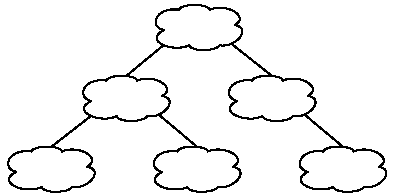
\includegraphics[width=2.2cm]{../img/tree.pdf} \\
\Emph{Graf}  & 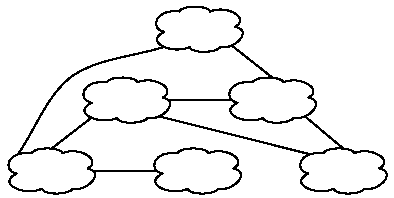
\includegraphics[width=2.2cm]{../img/graph.pdf} \\
\end{tabular}
\end{itemize}
{
\SlideFontTiny \vspace{1em }\hskip2em
Mer om listor \& träd \href{http://cs.lth.se/edaa01vt}{fördjupningskursen}. 
Mer om träd, grafer i \href{http://cs.lth.se/edaa40}{Diskreta strukturer.}
}

\end{Slide} 


\begin{Slide}{Vad är en vektor?}\SlideFontSmall
En \Emph{vektor}\footnote{Vektor kallas ibland på svenska även \href{https://sv.wikipedia.org/wiki/F\%C3\%A4lt_\%28datastruktur\%29}{fält}, men det skapar stor förvirring eftersom det engelska ordet \emph{field} ofta används för \emph{attribut} (förklaras senare).} 
\Eng{vector, \href{https://en.wikipedia.org/wiki/Array_data_structure}{array}} är en \Emph{samling} som är \Alert{snabb} att \Emph{indexera} i. 
Åtkomst av element sker med \code{apply(platsnummer)}: 

\begin{REPL}
scala> val heltal = Vector(42, 13, -1, 0 , 1)
heltal: scala.collection.immutable.Vector[Int] = Vector(42, 13, -1, 0, 1)

scala> heltal.apply(0)
res0: Int = 42

scala> heltal(1)    // man kan skippa .apply
res1: Int = 13

scala> heltal(5)
java.lang.IndexOutOfBoundsException: 5
  at scala.collection.immutable.Vector.checkRangeConvert(Vector.scala:132)
\end{REPL}
Utelämnar du \code{.apply} så gör kompilatorn anrop av \code{apply} ändå om det går.
\end{Slide}

\begin{Slide}{En konceptuell bild av en vektor}

\begin{REPLnonum}
scala> val heltal = Vector(42, 13, -1, 0 , 1)

scala> heltal(0)
res0: Int = 42
\end{REPLnonum}

\begin{tikzpicture}[font=\ttfamily]
\matrix [matrix of nodes, row sep=0, column 2/.style={nodes={rectangle,draw,minimum width=3em}}] (var) at (0cm, 2.8cm)
{
heltal   &  \makebox(16,12){ }\\
};
\matrix [matrix of nodes, draw=black,row sep=0, column 2/.style={nodes={rectangle,draw,minimum width=4em}}] (vec) at (4cm, 1cm)
{
\textit{plats} &  \\
0   &  \makebox(16,12){42}\\
1   &  \makebox(16,12){13}\\
2   &  \makebox(16,12){-1}\\
3   &  \makebox(16,12){0}\\
4   &  \makebox(16,12){1}\\
};
\filldraw[black] (0.7cm,2.8cm) circle (3pt) node[] (ref) {};
 \draw [arrow] (ref) -- (vec);
\end{tikzpicture}

%\vspace{1em} Elementen ligger på rad någonstans i minnet.
\end{Slide}



\begin{Slide}{En samling strängar}

\begin{itemize}
\item En vektor kan lagra många värden av samma typ. 
\item Elementen kan vara till exempel heltal eller strängar. 
\item Eller faktiskt vad som helst. 
\end{itemize}

\begin{REPL}
scala> val grönsaker = Vector("gurka","tomat","paprika","selleri")
grönsaker: scala.collection.immutable.Vector[String] = Vector(gurka, tomat, paprika, selleri)

scala> val g = grönsaker(1)
g: String = tomat

scala> val xs = Vector(42, "gurka", true, 42.0)
xs: scala.collection.immutable.Vector[Any] = Vector(42, gurka, true, 42.0)


\end{REPL}

\end{Slide}

\begin{Slide}{Vad är en kontrollstruktur?}
\begin{itemize}
\item En \Emph{kontrollstruktur} påverkar \Alert{sekvensen}.
\begin{itemize}
\item[] Exempel på inbyggda kontrollstrukturer: 
\\\vspace{0.5em}\code{for}-sats, \code{while}-sats
\end{itemize}

\item[]

\item I Scala kan man definiera \Emph{egna} kontrollstrukturer.
\begin{itemize}
\item[] Exempel: \code{upprepa} som du använt i Kojo
\\\vspace{0.5em}\code|upprepa(4){fram; höger}|
\end{itemize}
\end{itemize}
\end{Slide}


\begin{Slide}{Mitt första program: en oändlig loop på ABC80}
\begin{columns}
\begin{column}{0.8\textwidth}
\begin{verbatim}
10 print "hej"
20 goto 10
\end{verbatim}
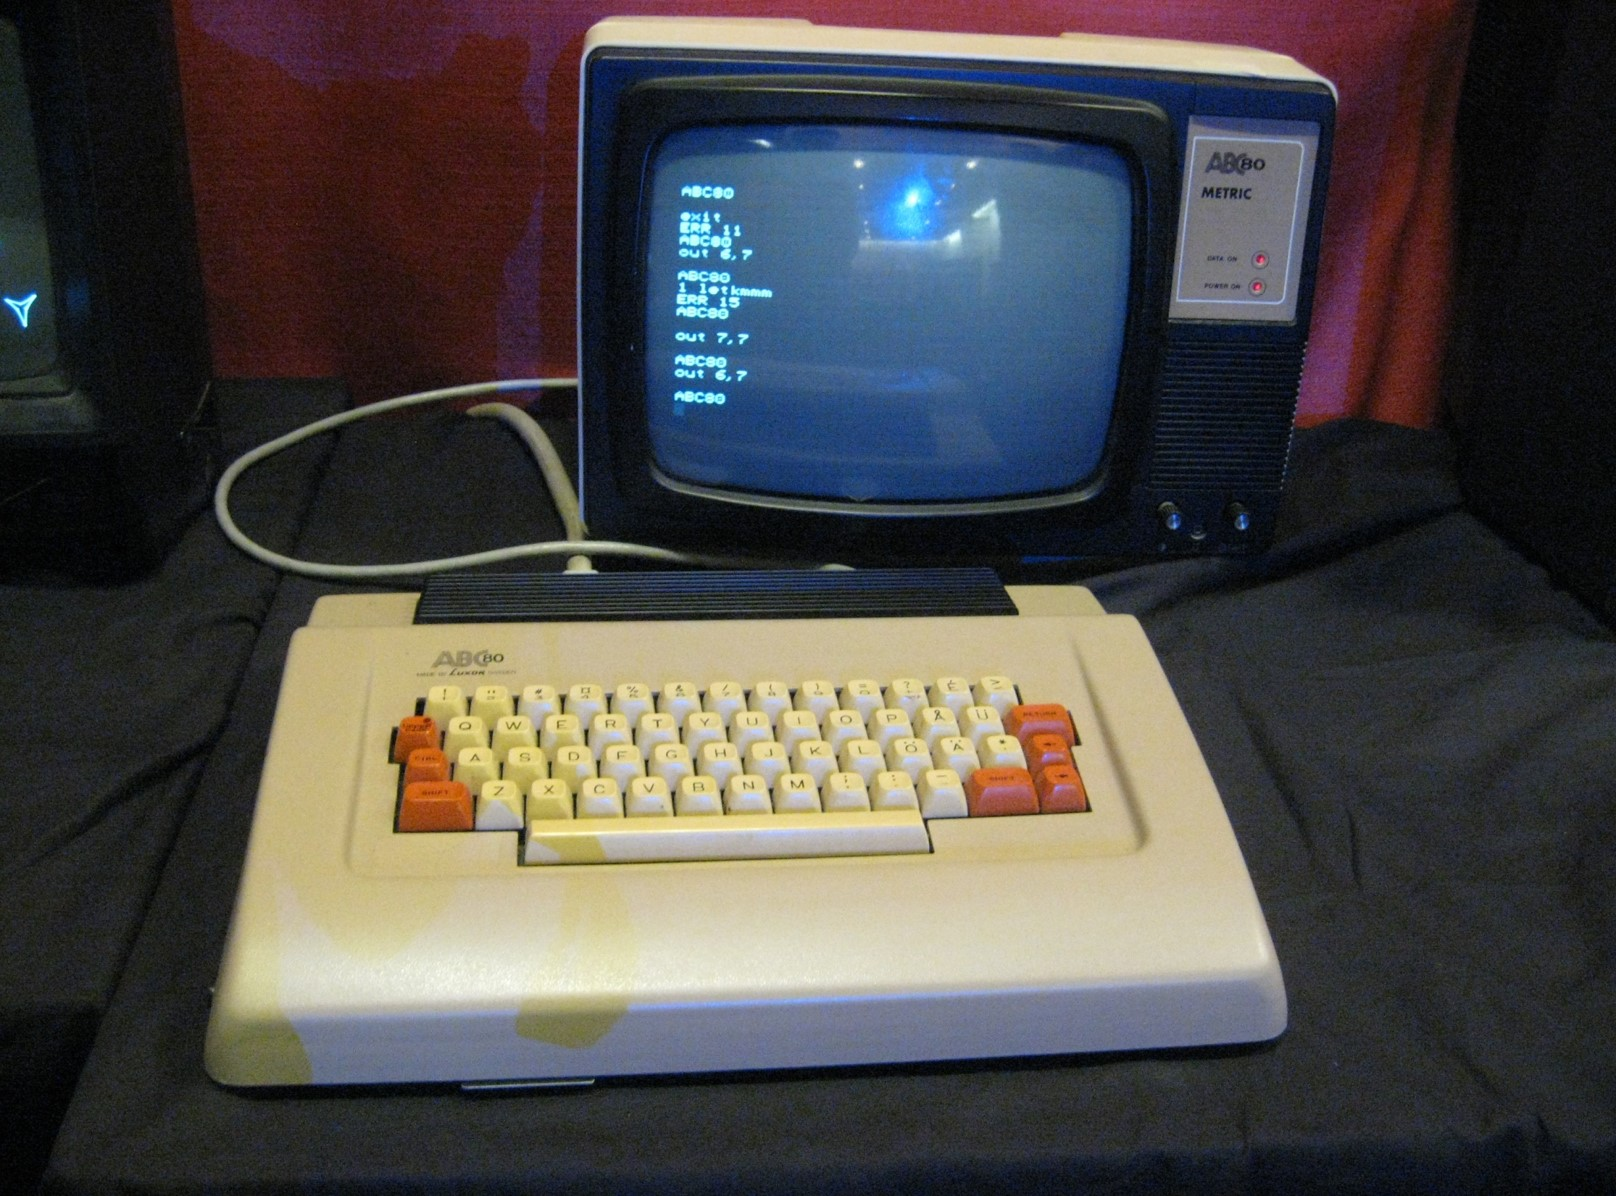
\includegraphics[width=0.8\textwidth]{../img/abc80.jpg}
\end{column}
\begin{column}{0.3\textwidth}
\pause
\begin{verbatim}
hej
hej
hej
hej
hej
hej
hej
hej
hej
hej
hej
hej
<Ctrl+C>
\end{verbatim}

\end{column}
\end{columns}
\end{Slide}


\begin{Slide}{Loopa genom elementen i en vektor}
En \code{for}-\Emph{sats} som skriver ut alla element i en vektor:
\begin{REPL}
scala> val grönsaker = Vector("gurka","tomat","paprika","selleri")

scala> for (g <- grönsaker) println(g)
gurka
tomat
paprika
selleri

\end{REPL}

\end{Slide}


\begin{Slide}{Bygga en ny samling från en befintlig med for-uttryck}
Ett \code{for}-\code{yield}-\Emph{uttryck} som \Emph{skapar en \Alert{ny} samling}.

\begin{Code}[basicstyle=\ttfamily\fontsize{12}{14}\selectfont]
for (g <- grönsaker) yield "god " + g
\end{Code}

\begin{REPL}
scala> val grönsaker = Vector("gurka","tomat","paprika","selleri")

scala> for (g <- grönsaker) yield "god " + g
res0: scala.collection.immutable.Vector[String] = 
  Vector(god gurka, god tomat, god paprika, god selleri)

scala> val åsikter = for (g <- grönsaker) yield s"god $g"
åsikter: scala.collection.immutable.Vector[String] = 
  Vector(god gurka, god tomat, god paprika, god selleri)
\end{REPL}

\end{Slide}


\begin{Slide}{Samlingen \code{Range} håller reda på intervall}
\begin{itemize}
\item Med en \code{Range(start, slut)} kan du skapa ett intervall: \\ från och med \code{start} till (men inte med) \code{slut}
\end{itemize}

\begin{REPLnonum}
scala> Range(0, 42)
res0: scala.collection.immutable.Range = 
  Range(0, 1, 2, 3, 4, 5, 6, 7, 8, 9, 10, 11, 12, 13, 14, 
    15, 16, 17, 18, 19, 20, 21, 22, 23, 24, 25, 26, 27, 28, 
    29, 30, 31, 32, 33, 34, 35, 36, 37, 38, 39, 40, 41)
\end{REPLnonum}

\begin{itemize}
\item Men alla värden däremellan skapas inte förrän de behövs:
\end{itemize}

\begin{REPL}
scala> val jättestortIntervall = Range(0, Int.MaxValue)
jättestortIntervall: scala.collection.immutable.Range = Range(0, 1, 2, 3, 4, 5, ...

scala> jättestortIntervall.end
res1: Int = 2147483647

scala> jättestortIntervall.toVector
java.lang.OutOfMemoryError: GC overhead limit exceeded
\end{REPL}

\end{Slide}

\begin{Slide}{Loopa med Range}
\code{Range} används i for-lopar för att hålla reda på antalet rundor.
\begin{REPLnonum}
scala> for (i <- Range(0, 6)) print(" gurka " + i)
 gurka 0 gurka 1 gurka 2 gurka 3 gurka 4 gurka 5 
\end{REPLnonum}
Du kan skapa en \code{Range} med \code{until} efter ett heltal:
\begin{REPLnonum}
scala> 1 until 7
res1: scala.collection.immutable.Range = 
  Range(1, 2, 3, 4, 5, 6)

scala> for (i <- 1 until 7) print(" tomat " + i) 
 tomat 1 tomat 2 tomat 3 tomat 4 tomat 5 tomat 6

\end{REPLnonum}
\end{Slide}

\begin{Slide}{Loopa med Range skapad med \texttt{to}}

Med \code{to} efter ett heltal får du en \code{Range} till och \Emph{med} sista:
\begin{REPLnonum}
scala> 1 to 6
res2: scala.collection.immutable.Range.Inclusive = 
  Range(1, 2, 3, 4, 5, 6)

scala> for (i <- 1 to 6) print(" gurka " + i) 
 gurka 1 gurka 2 gurka 3 gurka 4 gurka 5 gurka 6
 
\end{REPLnonum}


\end{Slide}



\begin{Slide}{Vad är en \code{Array} i JVM?}


\begin{itemize}
\item En \code{Array} liknar en \code{Vector} men har en särställning i JVM:
\begin{itemize}
\item Lagras som en sekvens i minnet på efterföljande adresser.
\item \Emph{Fördel}: snabbaste samlingen för element-access i JVM.
\item Men det finns en hel del \Alert{nackdelar} som vi ska se senare.
\end{itemize}

\end{itemize}

\begin{REPLnonum}
scala> val heltal = Array(42, 13, -1, 0 , 1)
\end{REPLnonum}

\begin{tikzpicture}[font=\ttfamily,scale=0.75, every node/.style={scale=0.75}]
\matrix [matrix of nodes, row sep=0, column 2/.style={nodes={rectangle,draw,minimum width=3em}}] (var) at (0cm, 2.8cm)
{
heltal   &  \makebox(16,12){ }\\
};
\matrix [matrix of nodes, draw=black,row sep=0, column 2/.style={nodes={rectangle,draw,minimum width=4em}}] (vec) at (4cm, 1cm)
{
\textit{plats} &  \\
0   &  \makebox(16,12){42}\\
1   &  \makebox(16,12){13}\\
2   &  \makebox(16,12){-1}\\
3   &  \makebox(16,12){0}\\
4   &  \makebox(16,12){1}\\
};
\filldraw[black] (0.7cm,2.8cm) circle (3pt) node[] (ref) {};
 \draw [arrow] (ref) -- (vec);
\end{tikzpicture}
\end{Slide}

\begin{Slide}{Några likheter \& skillnader mellan \texttt{Vector} och \texttt{Array}}\SlideFontSmall
\begin{multicols}{2}
\begin{REPL}[numbers=none]
scala> val xs = Vector(1,2,3)
\end{REPL}

\columnbreak

\begin{REPL}[numbers=none]
scala> val xs = Array(1,2,3)
\end{REPL}
\end{multicols}


Några likheter mellan \texttt{Vector} och \texttt{Array}
\begin{itemize}
\item Båda är samlingar som kan innehålla många element.

\item Med båda kan man snabbt accessa vilket element som helst: \code{xs(2)}

\item Båda har en fix storlek efter allokering.
\end{itemize}

Några viktiga skillnader:
\begin{multicols}{2}
\Emph{Vector}
\begin{itemize}
\item Är \Emph{oföränderlig}: du kan lita på att elementreferenserna aldrig någonsin kommer att ändras.

\item Är \Emph{snabb på att skapa en delvis förändrad kopia}, t.ex. tillägg/borttagning/uppdatering mitt i sekvensen.

\end{itemize}


\columnbreak

\Alert{Array}
\begin{itemize}
\item Är \Alert{föränderlig}: \code{xs(2) = 42}

\item Är \Alert{snabb} om man bara vill läsa eller skriva på befintliga platser.

\item Är \Alert{långsam} om man vill lägga till eller ta bort element mitt i sekvensen.

\end{itemize}
\end{multicols}
\end{Slide}



\Subsection{Huvudprogram med \texttt{main} i Scala och Java}

\begin{Slide}{Ett minimalt fristående program i Scala och Java}
Nedan Scala-kod skrivs i en editor, spara med valfritt filnamn:
\begin{Code}
// this is Scala 

object Hello {
  def main(args: Array[String]): Unit = {
    println("Hejsan scala-appen!")
  }
}
\end{Code}

\pause
\vspace{1em}
Nedan Java-kod skrivs i en editor, filen \Alert{måste} heta \texttt{Hi.java}

\begin{Code}[language=Java]
// this is Java 

public class Hi {
    public static void main(String[] args) {
        System.out.println("Hejsan Java-appen!");
    }
}
\end{Code}

\end{Slide}


\begin{Slide}{Loopa genom en samling med en \texttt{while}-sats}
\begin{REPLnonum}
scala> val xs = Vector("Hej","på","dej","!!!")
xs: scala.collection.immutable.Vector[String] = 
  Vector(Hej, på, dej, !!!)

scala> xs.size
res0: Int = 4

scala> var i = 0
i: Int = 0

scala> while (i < xs.size) { println(xs(i)); i = i + 1 }
Hej
på
dej
!!!
\end{REPLnonum}
\end{Slide}


\begin{Slide}{Loopa genom argumenten i ett Scala-huvudprogram}
Skriv denna kod och spara i filen \texttt{helloargs.scala}
\begin{REPL}[numbers=none]
$ gedit helloargs.scala
\end{REPL}
\begin{Code}
object HelloScalaArgs {
  def main(args: Array[String]): Unit = {
    var i = 0
    while (i < args.size) { 
      println(args(i))
      i = i + 1
    }
  }
}
\end{Code}
Kompilera och kör:
\begin{REPL}
$ scalac helloargs.scala
$ scala HelloScalaArgs hej gurka tomat 
hej
gurka
tomat
\end{REPL}
\end{Slide}


\begin{Slide}{Loopa genom argumenten i ett Java-huvudprogram}
\begin{REPL}[numbers=none]
$ gedit HelloJavaArgs.java
\end{REPL}
\begin{Code}[language=Java]
// this is Java 

public class HelloJavaArgs {
    public static void main(String[] args) {
    int i = 0;
    while (i < args.length) { 
      System.out.println(args[i]);
      i = i + 1;
    }
  }
}
\end{Code}
Kompilera och kör:
\begin{REPL}
$ javac HelloJavaArgs.scala
$ java HelloJavaArgs hej gurka tomat 
hej
gurka
tomat
\end{REPL}

\end{Slide}


\begin{Slide}{Scala-skript}
\begin{itemize}
\item Skala-kod kan köras som ett \Emph{skript}.\footnote{\SlideFontTiny Du får prova detta på övningen. Vi kommer mest att köra kompilerat i kursen, då Scala-skript saknar mekanism för inkludering av andra skript. Men det finns ett öppenkällkodsprojekt som löser det: \url{http://www.lihaoyi.com/Ammonite/}
}
\item Ett skript kompileras varje gång innan det körs och maskinkoden sparas inte som vid vanlig kompilering.
\item Då behövs ingen \code{main} och inget \code{object}
\end{itemize}

\begin{Code}[basicstyle=\ttfamily\fontsize{10}{12}\selectfont]
// spara nedan i filen 'myscript.scala'

println("Hejsan argumnet!")
for (arg <- args) println(arg)
\end{Code}

\begin{REPLnonum}
$ scala myscript.scala
\end{REPLnonum}


\end{Slide}



\Subsection{Algoritmer: stegvisa lösningar}

\begin{Slide}{Vad är en algoritm?}
En \href{https://sv.wikipedia.org/wiki/Algoritm}{algoritm} är en sekvens av instruktioner som beskriver \\hur man löser ett problem.\\
\vspace{1em}
\Emph{Exempel}: 
\begin{itemize}
\item	 baka en kaka 
\pause\item räkna ut din pensionsprognos 
\pause\item köra bil 
\pause\item kolla om highscore i ett spel 
\item ...
\end{itemize}

\begin{tikzpicture}[overlay]
\node[xshift=0.85\textwidth, scale=2.0] at (0,1.3) { 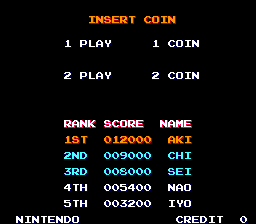
\includegraphics[width=0.25\textwidth]{../img/highscore}};
\end{tikzpicture}
\end{Slide}



\begin{Slide}{Algoritm-exempel: HIGHSCORE}
\Emph{Problem}: Kolla om high-score i ett spel \\ \vspace{1em}

\Emph{Varför?} \pause Så att de som spelar uppmuntras att spela mer :) \\ \vspace{1em}

\Emph{Algoritm:}\pause
\begin{enumerate}
\item $points$ $\leftarrow$ poängen efter senaste spelet
\item $highscore$ $\leftarrow$ bästa resultatet innan senaste spelet
\item \Key{om} $points$ är större än $highscore$ 
\begin{enumerate}[ ~~]
\item  Skriv ''Försök igen!''
\end{enumerate}
\Key{annars}
\begin{enumerate}[ ~~]
\item  Skriv ''Grattis!''
\end{enumerate}
\end{enumerate}
\pause
\scriptsize \Alert{Hittar du buggen?}
\end{Slide}


\begin{Slide}{HIGHSCORE implementerad i Scala}
\begin{Code}
import scala.io.StdIn.readLine

object HighScore {
  def main(args: Array[String]): Unit = {
    val points = readLine("Hur mång poäng fick du?").toInt
    val highscore = readLine("Vad var highscore före senaste spelet?").toInt
    val msg = if (points > highscore) "GRATTIS!" else "Försök igen!"
    println(msg) 
  }
}
\end{Code}
\pause
Är det en bugg eller en feature att det står\\ \texttt{points > highscore} \\ och inte \\ \texttt{points >= highscore} \\ ?
% Buggen är att man inte får GRATTIS om poäng == highscore vilket är tråkigt :)
\end{Slide}


\begin{Slide}{HIGHSCORE implementerad i Java}
\begin{Code}[language=Java]
import java.util.Scanner;

public class HighScore {
    public static void main(String[] args){
        Scanner scan = new Scanner(System.in);
        System.out.println("Hur många poäng fick du?");
        int points =  scan.nextInt();
        System.out.println("Vad var higscore före senaste spelet?");
        int highscore = scan.nextInt();
        if (points > highscore) {
            System.out.println("GRATTIS!");
        } else {
            System.out.println("Försök igen!");
        }
    }
}
\end{Code}
\end{Slide}


\begin{Slide}{Algoritmexempel: N-FAKULTET}
\begin{algorithm}[H]
 \SetKwInOut{Input}{Indata}\SetKwInOut{Output}{Resultat}

 \Input{heltalet $n$}
 \Output{utskrift av produkten av de första $n$ heltalen }
 ~\\
 $prod \leftarrow 1$ \\
 $i \leftarrow 2$  \\
 \While{$i \leq n$}{
  $prod \leftarrow prod * i$\\
  $i \leftarrow i + 1$
 }
 skriv ut $prod$
\end{algorithm}
\pause\vspace{1em}
\begin{itemize}\SlideFontSmall
\item Vad händer om $n$ är noll?
\item Vad händer om $n$ är ett?
\item Vad händer om $n$ är två?
\item Vad händer om $n$ är tre?
\end{itemize}
\end{Slide}

\begin{Slide}{Algoritmexempel: MIN}
\begin{algorithm}[H]
 \SetKwInOut{Input}{Indata}\SetKwInOut{Output}{Resultat}

 \Input{Array $args$ med strängar som alla innehåller heltal}
 \Output{utskrift av minsta heltalet }
 ~\\
 $min \leftarrow$ det största heltalet som kan uppkomma  \\
 $n \leftarrow $ antalet heltal \\
 $i \leftarrow 0$ \\
 \While{$i < n$}{
   $x \leftarrow args(i).toInt$ \\
   \If{( x < $min$)}{$min \leftarrow x$}
   $i \leftarrow i + 1$
 }
 skriv ut $min$
\end{algorithm}
\pause{\hfill \SlideFontTiny \Emph{Test med indata}: \code{args = Array("2", "42", "1", "2")}}
\end{Slide}


\Subsection{Funktioner skapar struktur}

\begin{Slide}{Mall för funktionsdefinitioner}

\code{def} funktionsnamn(parameterdeklarationer): returtyp = block

\pause\vspace{0.5em}\Emph{Exempel}:

\begin{Code}[basicstyle=\ttfamily\fontsize{9}{11}\selectfont]
def öka(i: Int): Int = { i + 1 }
\end{Code}
\pause Om ett enda uttryck: behövs inga \code|{}|. Returtypen kan härledas.
\begin{Code}[basicstyle=\ttfamily\fontsize{9}{11}\selectfont]
def öka(i: Int) = i + 1  
\end{Code}
\pause Om flera parametrar, separera dem med kommatecken: 
\begin{Code}[basicstyle=\ttfamily\fontsize{9}{11}\selectfont]
def isHighscore(points: Int, high: Int): Boolean = {
  val highscore: Boolean = points > high
  if (highscore) println(":)") else print(":(")
  highscore
}
\end{Code}
\pause Ovan funktion har \Alert{sidoeffekten} att skriva ut en smiley.
\end{Slide}

\begin{Slide}{Bättre många små abstraktioner som gör en sak var}

\begin{Code}[basicstyle=\ttfamily\fontsize{8}{11}\selectfont]
def isHighscore(points: Int, high: Int): Boolean = points > high

def printSmiley(isHappy: Boolean): Unit = 
  if (isHappy) println(":)") else print(":(")
\end{Code}

\pause\vspace{2em}
\begin{REPLnonum}
  printSmiley(isHighscore(113,99))
\end{REPLnonum}

\pause\vspace{2em} \code{isHigscore} är en \Emph{äkta funktion} som alltid ger samma svar för samma inparametrar och saknar \Alert{sidoeffekter}.

\end{Slide}



\begin{Slide}{Vad är ett block?}

\begin{itemize}
\item Ett block \Emph{kapslar in} flera satser/uttryck och ser ''utifrån'' ut som en enda sats/uttryck.

\item Ett block skapas med hjälp av klammerparenteser (''krullparenteser'')

\item [] {\fontsize{14}{18}\selectfont \code|{ uttryck1; uttryck2; ... uttryckN }|}\\~

\pause

\item I Scala (till skillnad från många andra språk) har ett block ett \Emph{värde} och är alltså ett \Emph{uttryck}. 

\item Värdet ges av \Emph{sista uttrycket}.

\begin{REPLnonum}
scala> val x = { println(1 + 1); println(2 + 2); 3 + 3 } 
2
4
x: Int = 6
\end{REPLnonum}


\end{itemize}

\end{Slide}

\begin{Slide}{Namn i block blir \textbf{lokala}}
Synlighetsregler: 
\begin{enumerate}
\item Identifierare deklarerade inuti ett block blir \Emph{lokala}.

\item Lokala namn \Alert{överskuggar} namn i yttre block om samma.


\item Namn syns i nästlade underblock.

\end{enumerate}

\begin{REPL}
scala> { val lokaltNamn = 42; println(lokaltNamn) }
42

scala> println(lokaltNamn)
<console>:12: error: not found: value lokaltNamn
       println(lokaltNamn)

scala> { val x = 42; { val x = 76; println(x) }; println(x) }
76
42

scala> { val x = 42; { val y = x + 1; println(y) } }
43
\end{REPL}

\end{Slide}


\begin{Slide}{Parameter och argument}

Skilj på parameter och argument!
\begin{itemize}
\item En \Alert{parameter} är det deklarerade namnet som används \Alert{lokalt} i en funktion för att referera till...

\item \Emph{argumentet} som är värdet som skickas med \Emph{vid anrop} och binds till det lokala parameternamnet.

\end{itemize}


\begin{REPLnonum}
scala> val ettArgument = 42

scala> def öka(minParameter: Int) = minParameter + 1

scala> öka(ettArgument)
\end{REPLnonum}


Speciell syntax: anrop med s.k. \Emph{namngiven parameter}
\begin{REPLnonum}
scala> öka(minParameter = ettArgument) 
\end{REPLnonum}

\end{Slide}

\begin{Slide}{Procedurer}\SlideFontSmall
\begin{itemize}
\item En \Emph{procedur} är en funktion som \Alert{gör} något intressant, men som \Alert{inte} lämnar något intressant returvärde.
\item Exempel på befintlig procedur: \code{println("hej")}
\item Du \Emph{deklarerar egna procedurer} genom att ange \texttt{\Alert{Unit}} som returvärdestyp. Då ges värdet \texttt{\Alert{()}} som betyder ''inget''.
\end{itemize}
\begin{REPL}
scala> def hej(x: String): Unit = println(s"Hej på dej $x!")
hej: (x: String)Unit

scala> hej("Herr Gurka")
Hej på dej Herr Gurka!

scala> val x = hej("Fru Tomat")
Hej på dej Fru Tomat!
x: Unit = ()
\end{REPL}
\begin{itemize}
\item Det som \Alert{görs} kallas (sido)\Emph{effekt}. Ovan är utskriften själva effekten.
\item Funktioner kan också ha sidoeffekter. De kallas då \Alert{oäkta} funktioner.
\end{itemize}
\end{Slide}

\begin{Slide}{''Ingenting'' \emph{är} faktiskt någonting i Scala}
\begin{itemize}
\item I många språk (Java, C, C++, ...) är funktioner som saknar värden speciella.
 Java m.fl. har speciell syntax för procedurer med nyckelordet \jcode{void}, men \Alert{inte} Scala. 

\item I Scala är procedurer inte specialfall; de är vanliga funktioner som returnerar ett värde som \Emph{representerar} ingenting, nämligen () som är av typen Unit. 

\item På så sätt blir procedurer inget undantag utan följer vanlig syntax och semantik precis som för alla andra funktioner.

\item Detta är typiskt för Scala: generalisera koncepten och vi slipper besvärliga undantag! \\(Men vi måste förstå generaliseringen...)


\item [] {\SlideFontSmall 
\url{https://en.wikipedia.org/wiki/Void_type}
\url{https://en.wikipedia.org/wiki/Unit_type}
}

\end{itemize}

\end{Slide}

\begin{Slide}{Abstraktion: Problemlösning genom nedbrytning i enkla funktioner och procedurer som kombineras}\SlideFontSmall
\begin{itemize}
\item En av de allra viktigaste principerna inom programmering är \Emph{funktionell nedbrytning} där  \Emph{underprogram} i form av funktioner och procedurer skapas för att bli byggstenar som kombineras till mer avancerade funktioner och procedurer.

\item Genom de namn som definieras skapas \Emph{återanvändbara abstraktioner} som kapslar in det funktionen gör. 

\item Problemet blir med bra byggblock lättare att lösa.

\item Abstraktioner som beräknar eller gör \Emph{en enda, väldefinierad sak} är enklare att använda, jämfört med de som gör många, helt olika saker.

\item Abstraktioner med \Emph{välgenomtänkta namn} är enklare att använda, jämfört med kryptiska eller missvisande namn.
\end{itemize}

\end{Slide}



\begin{Slide}{Exempel på \textbf{funktionell nedbrytning}}

Kojo-labben gav exempel på \Emph{funktionell nedbrytning} där ett antal abstraktioner skapas och återanvänds.

\begin{Code}
// skapa abstraktioner som bygger på varandra

def kvadrat = upprepa(4){fram; höger}

def stapel = {
  upprepa(10){kvadrat; hoppa}
  hoppa(-10*25)
}

def rutnät = upprepa(10){stapel; höger; fram; vänster}

// huvudprogram 

sudda; sakta(200)
rutnät
\end{Code}
\end{Slide}


\begin{Slide}{Varför abstraktion?}
\begin{itemize}
\item Stora program behöver delas upp annars blir det mycket svårt att förstå och bygga vidare på programmet.
\item Vi behöver kunna välja namn på saker i koden \textit{lokalt}, utan att det krockar med samma namn i andra delar av koden.
\item Abstraktioner hjälper till att hantera och kapsla in komplexa delar så att de blir enklare att använda om och om igen. 

\item Exempel på \Emph{abstraktionsmekanismer} i Scala och Java:
\begin{itemize}

\item \href{https://sv.wikipedia.org/wiki/Klass_\%28programmering\%29}{Klasser} är ''byggblock'' med kod som används för att skapa \href{https://sv.wikipedia.org/wiki/Objektorienterad_programmering\#Objekt}{objekt}, innehållande delar som hör ihop. \\ Nyckelord: \code{class} och \code{object} 

\item \href{https://en.wikipedia.org/wiki/Method_\%28computer_programming\%29}{Metoder} är funktioner som finns i klasser/objekt och används för att lösa specifika uppgifter.  Nyckelord: \code{def}

\item \href{https://en.wikipedia.org/wiki/Java_package}{Paket} används för att organisera kodfiler i en hierarkisk katalogstruktur och skapa namnrymder. \\Nyckelord: \Key{package}

\end{itemize}

\end{itemize}
\end{Slide}


\Subsection{Katalogstruktur för kodfiler med paket}



\begin{Slide}{Källkodsfiler och klassfiler}
\begin{tikzpicture}[node distance=1.5cm]
\node (input) [startstop] {\texttt{Hello.scala}};
\node(inptext) [right of=input, text width=5cm, scale=1.2,xshift=3.5cm]{Källkodsfil};
\node (compile) [process, below of=input] {\texttt{scalac}};
\node (output) [startstop, below of=compile] {\texttt{Hello.class}};
\node(outtext) [right of=output, text width=5cm, scale=1.2,xshift=3.5cm]{\texttt{.class}-fil med byte-kod};
\node (jvm) [process, below of=output] {JVM};
\node(jvmtext) [right of=jvm, text width=5.5cm, scale=0.8,xshift=4.5cm]{\textit{Java Virtual Machine}\\Översätter till maskinkod\\ som passar din specifika CPU\\medan programmet kör};
\draw [arrow] (input) -- (compile);
\draw [arrow] (compile) -- (output);
\draw [arrow] (output) -- (jvm);
\end{tikzpicture}
\end{Slide}




\begin{Slide}{Paket}\SlideFontSmall
\begin{itemize}
\item Paket ger struktur åt kodfilerna. Bra om man har många kodfiler.

\item Byte-koden placeras av kompilatorn i kataloger enligt paketstrukturen.


\end{itemize}

\vspace{1em}
\begin{tikzpicture}[node distance=1.5cm,scale=0.8, every node/.style={transform shape}]
\node (input) [startstop] {\texttt{greeting/Hello.scala}};
\node(inptext) [right of=input, text width=4cm, scale=1.2,xshift=4.5cm]{\lstinline{package greeting}\\\lstinline{object Hello { ... }};
\node (compile) [process, below of=input] {\texttt{scalac  greeting/Hello.java}};
\node (output) [startstop, below of=compile] {\texttt{greeting/Hello.class}};
\node(outtext) [right of=output, text width=4cm, scale=1.2,xshift=4.5cm]{Paketens bytekod hamnar i katalog med samma namn som paketnamnet};
\node (jvm) [process, below of=output] {\texttt{scala greeting.Hello}};
\draw [arrow] (input) -- (compile);
\draw [arrow] (compile) -- (output);
\draw [arrow] (output) -- (jvm);
\end{tikzpicture}

{\SlideFontTiny\vspace{1em} Katalogstrukturen för källkoden måste i Java motsvara paketstrukturen, \\men inte i Scala. Dock kräver många IDE att så görs även för Scala.}
\end{Slide}

\begin{Slide}{Import}
Med hjälp av punktnotation kommer man åt innehåll i ett paket.\\
\begin{Code}
val age = scala.io.StdIn.readLine("Ange din ålder:")
\end{Code}

En \code{import}-sats...
 
\begin{Code}
import scala.io.StdIn.readLine
\end{Code}

...gör så att kompilatorn ''ser'' namnet, och man slipper skriva hela sökvägen till namnet:
\begin{Code}
val age = readLine("Ange din ålder:")
\end{Code}

Man säger att det importerade namnet hamnar \Emph{\textit{in scope}}.
\end{Slide}





\begin{Slide}{Jar-filer}
\texttt{jar}-filer liknar \texttt{zip}-filer och används för att packa ihop bytekod i en enda fil för enkel distribution och körning. 

\vspace{2em}
\begin{tikzpicture}[node distance=1.5cm,scale=0.8, every node/.style={transform shape}]
\node (input) [startstop] {\texttt{greeting/}};
\node(inptext) [right of=input, text width=4cm, scale=1.2,xshift=4.5cm]{en katalog med filer};
\node (jar) [process, below of=input] 
{\texttt{jar cvf minjarfil.jar greeting}};

\node (output) [startstop, below of=compile] {\texttt{minjarfil.jar}};

\node(outtext) [right of=output, text width=4cm, scale=1.2,xshift=4.5cm]{En jar-fil med alla filer inpackade};

\node (jvm) [process, below of=output] {\texttt{scala -cp minjarfil.jar}};

\node(outtextjvm) [right of=jvm, text width=4cm, scale=1.2,xshift=4.5cm]{Lägg jar-filen till \\ ''classpath''};
\draw [arrow] (input) -- (jar);
\draw [arrow] (jar) -- (output);
\draw [arrow] (output) -- (jvm);
\end{tikzpicture}
\end{Slide}

\Subsection{Dokumentation}

\begin{Slide}{Dokumentation}\footnotesize
För att kod ska bli begriplig för människor är det bra att dokumentera vad den gör. Det finns \Emph{tre olika sorters kommentarer} som man kan skriva direkt i Scala/Java-koden, \Alert{som kompilatorn struntar fullständigt i}:
\begin{lstlisting}
// Enradskommentarer börjar med dubbla snedstreck
//       men de gäller bara till radslut

/* Flerradskommentarer börjar med 
   snedstreck-asterisk
   och slutar med asterisk-snedstreck.  */ 

/** Dokumentationskommentarer placeras före 
 *   t.ex. en funktion och berättar vad den gör
 *   och vad eventuella parametrar används till.
 *   Börjar med snedstreck-asterisk-asterisk.
 *   Varje ny kommentarsrad börjar med asterisk.
 *   Avslutas med asterisk-stjärna.
 */
\end{lstlisting}
\end{Slide}

\begin{Slide}{scaladoc}
Programmet \texttt{scaladoc}-filer läser källkod och skapar en webbsajt med dokumentation. 

\vspace{2em}
\begin{tikzpicture}[node distance=1.5cm,scale=0.8, every node/.style={transform shape}]

\node (input) [startstop] {\texttt{greeting/}};

\node(inptext) [right of=input, text width=4cm, scale=1.2,xshift=4.5cm]{en katalog med \texttt{.scala}-filer};

\node (scaladoc) [process, below of=input] 
{\texttt{scaladoc greeting/*.scala}};

\node (output) [startstop, below of=compile] {\texttt{index.html} ~~med mera...};

\node(outtext) [right of=output, text width=4cm, scale=1.2,xshift=4.5cm]{En webbsajt};


\draw [arrow] (input) -- (scaladoc);
\draw [arrow] (scaladoc) -- (output);
\end{tikzpicture}
\end{Slide}



\subsection{Att göra denna vecka}


%%%
\begin{Slide}{Att göra i Vecka \vecka: Förstå grundläggande kodstrukturer}

\begin{enumerate}
\item Laborationer är \Alert{obligatoriska}.\\ Ev. sjukdom måste anmälas \Alert{före} via mejl till kursansvarig!
\item Gör övning \texttt{programs}
\item OBS! Ingen lab denna vecka w02. Använd tiden att komma ikapp om du ligger efter!
\item Träffas i samarbetsgrupper och hjälp varandra att förstå.
\item Vi har nosat på flera koncept som vi kommer tillbaka till senare: du måste inte fatta alla detaljer redan nu.
\item Om ni inte redan gjort det: \\Visa \href{https://github.com/bjornregnell/lth-eda016-2015/tree/master/assignments}{samarbetskontrakt} för handledare på resurstid.
\item \Alert{Koda på resurstiderna} och få hjälp och tips! 
\end{enumerate}
\end{Slide}

\begin{Slide}{Veckans övning: \code{w02-programs}}\SlideFontTiny
\vspace{-0.5em}
\setlength{\leftmargini}{0pt}
\begin{itemize}
%!TEX encoding = UTF-8 Unicode
%!TEX root = ../compendium2.tex

\item Kunna skapa samlingarna Range, Array och Vector med heltals- och strängvärden.
\item Kunna indexera i en indexerbar samling, t.ex. Array och Vector.
\item Kunna anropa operationerna size, mkString, sum, min, max på samlingar som innehåller heltal.
\item Känna till grundläggande skillnader och likheter mellan samlingarna Range, Array och Vector.
\item Förstå skillnaden mellan en for-sats och ett for-uttryck.
\item Kunna skapa samlingar med heltalsvärden som resultat av enkla for-uttryck.
\item Förstå skillnaden mellan en algoritm i pseudo-kod och dess implementation.
\item Kunna implementera algoritmerna SUM, MIN/MAX på en indexerbar samling med en \code{while}-sats.
\item Kunna köra igång enkel Scala-kod i REPL, som skript och som applikation.
\item Kunna skriva och köra igång ett enkelt Java-program.
\item Känna till några grundläggande syntaxskillnader mellan Scala och Java, speciellt variabeldeklarationer och indexering i Array.
\item Förstå vad ett block och en lokal variabel är.
\item Förstå hur nästlade block påverkar namnsynlighet och namnöverskuggning.
\item Förstå kopplingen mellan paketstruktur och kodfilstruktur.
\item Kunna skapa en jar-fil.
\item Kunna skapa dokumentation med scaladoc.

\end{itemize}
\end{Slide}













\end{document}
